\documentclass[twoside]{book}

% Packages required by doxygen
\usepackage{fixltx2e}
\usepackage{calc}
\usepackage{doxygen}
\usepackage[export]{adjustbox} % also loads graphicx
\usepackage{graphicx}
\usepackage[utf8]{inputenc}
\usepackage{makeidx}
\usepackage{multicol}
\usepackage{multirow}
\PassOptionsToPackage{warn}{textcomp}
\usepackage{textcomp}
\usepackage[nointegrals]{wasysym}
\usepackage[table]{xcolor}

% Font selection
\usepackage[T1]{fontenc}
\usepackage[scaled=.90]{helvet}
\usepackage{courier}
\usepackage{amssymb}
\usepackage{sectsty}
\renewcommand{\familydefault}{\sfdefault}
\allsectionsfont{%
  \fontseries{bc}\selectfont%
  \color{darkgray}%
}
\renewcommand{\DoxyLabelFont}{%
  \fontseries{bc}\selectfont%
  \color{darkgray}%
}
\newcommand{\+}{\discretionary{\mbox{\scriptsize$\hookleftarrow$}}{}{}}

% Page & text layout
\usepackage{geometry}
\geometry{%
  a4paper,%
  top=2.5cm,%
  bottom=2.5cm,%
  left=2.5cm,%
  right=2.5cm%
}
\tolerance=750
\hfuzz=15pt
\hbadness=750
\setlength{\emergencystretch}{15pt}
\setlength{\parindent}{0cm}
\setlength{\parskip}{3ex plus 2ex minus 2ex}
\makeatletter
\renewcommand{\paragraph}{%
  \@startsection{paragraph}{4}{0ex}{-1.0ex}{1.0ex}{%
    \normalfont\normalsize\bfseries\SS@parafont%
  }%
}
\renewcommand{\subparagraph}{%
  \@startsection{subparagraph}{5}{0ex}{-1.0ex}{1.0ex}{%
    \normalfont\normalsize\bfseries\SS@subparafont%
  }%
}
\makeatother

% Headers & footers
\usepackage{fancyhdr}
\pagestyle{fancyplain}
\fancyhead[LE]{\fancyplain{}{\bfseries\thepage}}
\fancyhead[CE]{\fancyplain{}{}}
\fancyhead[RE]{\fancyplain{}{\bfseries\leftmark}}
\fancyhead[LO]{\fancyplain{}{\bfseries\rightmark}}
\fancyhead[CO]{\fancyplain{}{}}
\fancyhead[RO]{\fancyplain{}{\bfseries\thepage}}
\fancyfoot[LE]{\fancyplain{}{}}
\fancyfoot[CE]{\fancyplain{}{}}
\fancyfoot[RE]{\fancyplain{}{\bfseries\scriptsize Generated by Doxygen }}
\fancyfoot[LO]{\fancyplain{}{\bfseries\scriptsize Generated by Doxygen }}
\fancyfoot[CO]{\fancyplain{}{}}
\fancyfoot[RO]{\fancyplain{}{}}
\renewcommand{\footrulewidth}{0.4pt}
\renewcommand{\chaptermark}[1]{%
  \markboth{#1}{}%
}
\renewcommand{\sectionmark}[1]{%
  \markright{\thesection\ #1}%
}

% Indices & bibliography
\usepackage{natbib}
\usepackage[titles]{tocloft}
\setcounter{tocdepth}{3}
\setcounter{secnumdepth}{5}
\makeindex

% Hyperlinks (required, but should be loaded last)
\usepackage{ifpdf}
\ifpdf
  \usepackage[pdftex,pagebackref=true]{hyperref}
\else
  \usepackage[ps2pdf,pagebackref=true]{hyperref}
\fi
\hypersetup{%
  colorlinks=true,%
  linkcolor=blue,%
  citecolor=blue,%
  unicode%
}

% Custom commands
\newcommand{\clearemptydoublepage}{%
  \newpage{\pagestyle{empty}\cleardoublepage}%
}

\usepackage{caption}
\captionsetup{labelsep=space,justification=centering,font={bf},singlelinecheck=off,skip=4pt,position=top}

%===== C O N T E N T S =====

\begin{document}

% Titlepage & ToC
\hypersetup{pageanchor=false,
             bookmarksnumbered=true,
             pdfencoding=unicode
            }
\pagenumbering{roman}
\begin{titlepage}
\vspace*{7cm}
\begin{center}%
{\Large Lane Detection }\\
\vspace*{1cm}
{\large Generated by Doxygen 1.8.11}\\
\end{center}
\end{titlepage}
\clearemptydoublepage
\tableofcontents
\clearemptydoublepage
\pagenumbering{arabic}
\hypersetup{pageanchor=true}

%--- Begin generated contents ---
\chapter{Class Index}
\section{Class List}
Here are the classes, structs, unions and interfaces with brief descriptions\+:\begin{DoxyCompactList}
\item\contentsline{section}{\hyperlink{classLane}{Lane} }{\pageref{classLane}}{}
\item\contentsline{section}{\hyperlink{classLaneDetectionModule}{Lane\+Detection\+Module} }{\pageref{classLaneDetectionModule}}{}
\end{DoxyCompactList}

\chapter{File Index}
\section{File List}
Here is a list of all documented files with brief descriptions\+:\begin{DoxyCompactList}
\item\contentsline{section}{/home/rohit/\+Opencv codes/\+Lane-\/\+Detection/include/\hyperlink{Lane_8hpp}{Lane.\+hpp} \\*\hyperlink{classLane}{Lane} Detection }{\pageref{Lane_8hpp}}{}
\item\contentsline{section}{/home/rohit/\+Opencv codes/\+Lane-\/\+Detection/include/{\bfseries Lane\+Detection\+Module.\+hpp} }{\pageref{LaneDetectionModule_8hpp}}{}
\item\contentsline{section}{/home/rohit/\+Opencv codes/\+Lane-\/\+Detection/test/\hyperlink{LaneDetectionModuleTest_8cpp}{Lane\+Detection\+Module\+Test.\+cpp} \\*Program to test \hyperlink{classLaneDetectionModule}{Lane\+Detection\+Module} class }{\pageref{LaneDetectionModuleTest_8cpp}}{}
\item\contentsline{section}{/home/rohit/\+Opencv codes/\+Lane-\/\+Detection/test/\hyperlink{LaneTest_8cpp}{Lane\+Test.\+cpp} \\*Program to test \hyperlink{classLaneDetectionModule}{Lane\+Detection\+Module} class }{\pageref{LaneTest_8cpp}}{}
\end{DoxyCompactList}

\chapter{Class Documentation}
\hypertarget{classLane}{}\section{Lane Class Reference}
\label{classLane}\index{Lane@{Lane}}
\subsection*{Public Member Functions}
\begin{DoxyCompactItemize}
\item 
\hyperlink{classLane_affd642d537d96c03cb7fe8c8d46d37b4}{Lane} ()\hypertarget{classLane_affd642d537d96c03cb7fe8c8d46d37b4}{}\label{classLane_affd642d537d96c03cb7fe8c8d46d37b4}

\begin{DoxyCompactList}\small\item\em Default constructor for \hyperlink{classLane}{Lane} with ployorder,colour,poly\+Coeff,start\+Coordinate,status random values. \end{DoxyCompactList}\item 
\hyperlink{classLane_a7dac966c4a38ff5440e70b2be72aa5ac}{Lane} (int poly\+Order, std\+::string color, int averaging\+Count)
\begin{DoxyCompactList}\small\item\em Default constructor for \hyperlink{classLane}{Lane} with ployorder,colour,poly\+Coeff,start\+Coordinate,status random values. \end{DoxyCompactList}\item 
\hyperlink{classLane_a1c023c4eca02fb9a52365b7f6c04d7d4}{$\sim$\+Lane} ()\hypertarget{classLane_a1c023c4eca02fb9a52365b7f6c04d7d4}{}\label{classLane_a1c023c4eca02fb9a52365b7f6c04d7d4}

\begin{DoxyCompactList}\small\item\em Default destructor for \hyperlink{classLane}{Lane} class. \end{DoxyCompactList}\item 
int {\bfseries get\+Stable\+Center} (int coordinate)\hypertarget{classLane_a6e8a964eef75687d6c18d847e87dd938}{}\label{classLane_a6e8a964eef75687d6c18d847e87dd938}

\item 
void {\bfseries set\+Start\+Coordinate} (cv\+::\+Point point)\hypertarget{classLane_a33adbdc77bb6c4bcaaec18cfcc1ab3d2}{}\label{classLane_a33adbdc77bb6c4bcaaec18cfcc1ab3d2}

\item 
cv\+::\+Point {\bfseries get\+Start\+Coordinate} ()\hypertarget{classLane_adb05103858eddf69b9f9edcf667ae92e}{}\label{classLane_adb05103858eddf69b9f9edcf667ae92e}

\item 
void {\bfseries set\+Status} (bool flag)\hypertarget{classLane_a826f43f6b4512ed0022c1b2d156eef9f}{}\label{classLane_a826f43f6b4512ed0022c1b2d156eef9f}

\item 
bool {\bfseries get\+Status} ()\hypertarget{classLane_a98690f0b93988f8c8fd58d3035b6c483}{}\label{classLane_a98690f0b93988f8c8fd58d3035b6c483}

\item 
void {\bfseries set\+Poly\+Order} (int value)\hypertarget{classLane_a8b15e2745d2634cd0b2d7a65e5310892}{}\label{classLane_a8b15e2745d2634cd0b2d7a65e5310892}

\item 
int {\bfseries get\+Poly\+Order} ()\hypertarget{classLane_ac0ff2db58a40689bc842edb120740632}{}\label{classLane_ac0ff2db58a40689bc842edb120740632}

\item 
void {\bfseries set\+Poly\+Coeff} (cv\+::\+Mat coeff)\hypertarget{classLane_a992415d3df4ed98dec71f5b5002becd7}{}\label{classLane_a992415d3df4ed98dec71f5b5002becd7}

\item 
std\+::vector$<$ float $>$ {\bfseries get\+Poly\+Coeff} ()\hypertarget{classLane_a4a433e238260f9464af03611c2a3d1ce}{}\label{classLane_a4a433e238260f9464af03611c2a3d1ce}

\end{DoxyCompactItemize}


\subsection{Constructor \& Destructor Documentation}
\index{Lane@{Lane}!Lane@{Lane}}
\index{Lane@{Lane}!Lane@{Lane}}
\subsubsection[{\texorpdfstring{Lane(int poly\+Order, std\+::string color, int averaging\+Count)}{Lane(int polyOrder, std::string color, int averagingCount)}}]{\setlength{\rightskip}{0pt plus 5cm}Lane\+::\+Lane (
\begin{DoxyParamCaption}
\item[{int}]{poly\+Order, }
\item[{std\+::string}]{color, }
\item[{int}]{averaging\+Count}
\end{DoxyParamCaption}
)}\hypertarget{classLane_a7dac966c4a38ff5440e70b2be72aa5ac}{}\label{classLane_a7dac966c4a38ff5440e70b2be72aa5ac}


Default constructor for \hyperlink{classLane}{Lane} with ployorder,colour,poly\+Coeff,start\+Coordinate,status random values. 


\begin{DoxyParams}{Parameters}
{\em poly\+Order} & is order of fitting polynomial \\
\hline
{\em color} & is the color of lane \\
\hline
{\em averaging\+Count} & number of values to average \\
\hline
\end{DoxyParams}


The documentation for this class was generated from the following file\+:\begin{DoxyCompactItemize}
\item 
/home/rohit/\+Opencv codes/\+Lane-\/\+Detection/include/\hyperlink{Lane_8hpp}{Lane.\+hpp}\end{DoxyCompactItemize}

\hypertarget{classLaneDetectionModule}{}\section{Lane\+Detection\+Module Class Reference}
\label{classLaneDetectionModule}\index{Lane\+Detection\+Module@{Lane\+Detection\+Module}}
\subsection*{Public Member Functions}
\begin{DoxyCompactItemize}
\item 
\hyperlink{classLaneDetectionModule_a044d95cfc95e4dba1c96ee62c50b6df6}{Lane\+Detection\+Module} ()\hypertarget{classLaneDetectionModule_a044d95cfc95e4dba1c96ee62c50b6df6}{}\label{classLaneDetectionModule_a044d95cfc95e4dba1c96ee62c50b6df6}

\begin{DoxyCompactList}\small\item\em Default constructor for \hyperlink{classLaneDetectionModule}{Lane\+Detection\+Module}. \end{DoxyCompactList}\item 
\hyperlink{classLaneDetectionModule_abe9179d4df794c39d6fe246ad7a0d64e}{$\sim$\+Lane\+Detection\+Module} ()\hypertarget{classLaneDetectionModule_abe9179d4df794c39d6fe246ad7a0d64e}{}\label{classLaneDetectionModule_abe9179d4df794c39d6fe246ad7a0d64e}

\begin{DoxyCompactList}\small\item\em Default destructor for \hyperlink{classLaneDetectionModule}{Lane\+Detection\+Module}. \end{DoxyCompactList}\item 
void \hyperlink{classLaneDetectionModule_aff46b8eb6123f639c84eabb574f03241}{undistort\+Image} (const cv\+::\+Mat \&src, cv\+::\+Mat \&dst)
\begin{DoxyCompactList}\small\item\em Method Undistortedimage for \hyperlink{classLaneDetectionModule}{Lane\+Detection\+Module}. \end{DoxyCompactList}\item 
void \hyperlink{classLaneDetectionModule_aca6f7ab235dcfd5f162ee3fd876a3f8a}{threshold\+ImageY} (const cv\+::\+Mat \&src, cv\+::\+Mat \&dst)
\begin{DoxyCompactList}\small\item\em Method threshold\+ImageY to set yellow threshold image for \hyperlink{classLaneDetectionModule}{Lane\+Detection\+Module}. \end{DoxyCompactList}\item 
void \hyperlink{classLaneDetectionModule_ae3478b6b12b994fdda59573ce1b9f57f}{threshold\+ImageW} (const cv\+::\+Mat \&src, cv\+::\+Mat \&dst)
\begin{DoxyCompactList}\small\item\em Method threshold\+ImageW to set white threshold image for \hyperlink{classLaneDetectionModule}{Lane\+Detection\+Module}. \end{DoxyCompactList}\item 
void \hyperlink{classLaneDetectionModule_ad05cacb2cac52d64ee0ab295dcbcd7af}{extract\+R\+OI} (const cv\+::\+Mat \&src, cv\+::\+Mat \&dst)
\begin{DoxyCompactList}\small\item\em Method extract\+R\+OI to set region of interest for \hyperlink{classLaneDetectionModule}{Lane\+Detection\+Module}. \end{DoxyCompactList}\item 
void \hyperlink{classLaneDetectionModule_a3b8c0ca214fbf200c25bd24194140afc}{transform\+Perspective} (const cv\+::\+Mat \&src, cv\+::\+Mat \&dst, cv\+::\+Mat \&Tm, cv\+::\+Mat \&inv\+Tm)
\begin{DoxyCompactList}\small\item\em Method transforming perspective of lane image. \end{DoxyCompactList}\item 
void \hyperlink{classLaneDetectionModule_aac3d46f14bbdbdea78991e84beff383e}{extract\+Lanes} (const cv\+::\+Mat \&src, cv\+::\+Mat \&dst, \hyperlink{classLane}{Lane} \&lane1, \hyperlink{classLane}{Lane} \&lane2, int curve\+Flag)
\begin{DoxyCompactList}\small\item\em Method extract\+Lanes to calculate parameters of lines and its characteristics for \hyperlink{classLaneDetectionModule}{Lane\+Detection\+Module}. \end{DoxyCompactList}\item 
void \hyperlink{classLaneDetectionModule_a9b982428acc3a1e83503c6e079ae3a50}{fit\+Poly} (const std\+::vector$<$ cv\+::\+Point $>$ \&src, cv\+::\+Mat \&dst, int order)
\begin{DoxyCompactList}\small\item\em Method fit\+Poly fits a 2nd order polynomial to the points on the lane. \end{DoxyCompactList}\item 
double \hyperlink{classLaneDetectionModule_a5a3cfd88512d1ce1e5dc55aed8d47e5f}{get\+Drive\+Heading} (\hyperlink{classLane}{Lane} \&lane1, \hyperlink{classLane}{Lane} \&lane2, std\+::string \&direction)
\begin{DoxyCompactList}\small\item\em Method get\+Drive\+Heading to calculate drive heading to be given to actuator for further action in \hyperlink{classLaneDetectionModule}{Lane\+Detection\+Module}. \end{DoxyCompactList}\item 
void \hyperlink{classLaneDetectionModule_a12af439407512c538f983508d98cf1f3}{display\+Output} (const cv\+::\+Mat \&src, cv\+::\+Mat \&src2, cv\+::\+Mat \&dst, \hyperlink{classLane}{Lane} \&lane1, \hyperlink{classLane}{Lane} \&lane2, cv\+::\+Mat inv)
\begin{DoxyCompactList}\small\item\em Method display\+Output to calculate to display of the system for \hyperlink{classLaneDetectionModule}{Lane\+Detection\+Module}. \end{DoxyCompactList}\item 
bool \hyperlink{classLaneDetectionModule_a7b98ab6e8187993381f2c69b03ca76ef}{detect\+Lane} (std\+::string video\+Name)
\begin{DoxyCompactList}\small\item\em Method detect\+Lane check if program is successfully running gives bool output for \hyperlink{classLaneDetectionModule}{Lane\+Detection\+Module}. \end{DoxyCompactList}\item 
cv\+::\+Scalar \hyperlink{classLaneDetectionModule_a6623e87aa620c98c782c03392ce77def}{get\+Yellow\+Max} ()
\begin{DoxyCompactList}\small\item\em Method get\+Yellow\+Max is to use get H\+SL max value of yellow for \hyperlink{classLaneDetectionModule}{Lane\+Detection\+Module}. \end{DoxyCompactList}\item 
cv\+::\+Scalar \hyperlink{classLaneDetectionModule_a9b31a2a27534fdefbcfb2de841a893c2}{get\+Yellow\+Min} ()
\begin{DoxyCompactList}\small\item\em Method get\+Yellow\+Min is to use get H\+SL min value of yellow for \hyperlink{classLaneDetectionModule}{Lane\+Detection\+Module}. \end{DoxyCompactList}\item 
void \hyperlink{classLaneDetectionModule_a1f1d6d0bc111273b359db4ef289beef7}{set\+Yellow\+Max} (cv\+::\+Scalar value)
\begin{DoxyCompactList}\small\item\em Method set\+Yellow\+Max is to use set H\+SL max value of yellow for \hyperlink{classLaneDetectionModule}{Lane\+Detection\+Module}. \end{DoxyCompactList}\item 
void \hyperlink{classLaneDetectionModule_a6d6f42b5de704c711f0bdcf39173871b}{set\+Yellow\+Min} (cv\+::\+Scalar value)
\begin{DoxyCompactList}\small\item\em Method set\+Yellow\+Min is to use set min value of yellow for \hyperlink{classLaneDetectionModule}{Lane\+Detection\+Module}. \end{DoxyCompactList}\item 
void \hyperlink{classLaneDetectionModule_a36183171cc012f8444a995b718b22efc}{set\+Gray\+Scale\+Max} (int value)
\begin{DoxyCompactList}\small\item\em Method set\+Gray\+Scale\+Max is to use set max value of Gray scale value for \hyperlink{classLaneDetectionModule}{Lane\+Detection\+Module}. \end{DoxyCompactList}\item 
void \hyperlink{classLaneDetectionModule_a2aaaf00d3570b863502363a473f143c5}{set\+Gray\+Scale\+Min} (int value)
\begin{DoxyCompactList}\small\item\em Method set\+Gray\+Scale\+Min is to use set min value of Gray scale value for \hyperlink{classLaneDetectionModule}{Lane\+Detection\+Module}. \end{DoxyCompactList}\item 
int \hyperlink{classLaneDetectionModule_a51c717f41ad97457213bbe2a079f3ece}{get\+Gray\+Scale\+Min} ()
\begin{DoxyCompactList}\small\item\em Method get\+Gray\+Scale\+Min is to use get min value of Gray\+Scale for \hyperlink{classLaneDetectionModule}{Lane\+Detection\+Module}. \end{DoxyCompactList}\item 
int \hyperlink{classLaneDetectionModule_a886adf9d2fdfac6f6f4794cb327ea73c}{get\+Gray\+Scale\+Max} ()
\begin{DoxyCompactList}\small\item\em Method get\+Gray\+Scale\+Max is to use get max value of Gray\+Scale for \hyperlink{classLaneDetectionModule}{Lane\+Detection\+Module}. \end{DoxyCompactList}\end{DoxyCompactItemize}


\subsection{Member Function Documentation}
\index{Lane\+Detection\+Module@{Lane\+Detection\+Module}!detect\+Lane@{detect\+Lane}}
\index{detect\+Lane@{detect\+Lane}!Lane\+Detection\+Module@{Lane\+Detection\+Module}}
\subsubsection[{\texorpdfstring{detect\+Lane(std\+::string video\+Name)}{detectLane(std::string videoName)}}]{\setlength{\rightskip}{0pt plus 5cm}bool Lane\+Detection\+Module\+::detect\+Lane (
\begin{DoxyParamCaption}
\item[{std\+::string}]{video\+Name}
\end{DoxyParamCaption}
)}\hypertarget{classLaneDetectionModule_a7b98ab6e8187993381f2c69b03ca76ef}{}\label{classLaneDetectionModule_a7b98ab6e8187993381f2c69b03ca76ef}


Method detect\+Lane check if program is successfully running gives bool output for \hyperlink{classLaneDetectionModule}{Lane\+Detection\+Module}. 


\begin{DoxyParams}{Parameters}
{\em video\+Name} & is video of source\\
\hline
\end{DoxyParams}
\begin{DoxyReturn}{Returns}
Status of lane detection. 
\end{DoxyReturn}
\index{Lane\+Detection\+Module@{Lane\+Detection\+Module}!display\+Output@{display\+Output}}
\index{display\+Output@{display\+Output}!Lane\+Detection\+Module@{Lane\+Detection\+Module}}
\subsubsection[{\texorpdfstring{display\+Output(const cv\+::\+Mat \&src, cv\+::\+Mat \&src2, cv\+::\+Mat \&dst, Lane \&lane1, Lane \&lane2, cv\+::\+Mat inv)}{displayOutput(const cv::Mat &src, cv::Mat &src2, cv::Mat &dst, Lane &lane1, Lane &lane2, cv::Mat inv)}}]{\setlength{\rightskip}{0pt plus 5cm}void Lane\+Detection\+Module\+::display\+Output (
\begin{DoxyParamCaption}
\item[{const cv\+::\+Mat \&}]{src, }
\item[{cv\+::\+Mat \&}]{src2, }
\item[{cv\+::\+Mat \&}]{dst, }
\item[{{\bf Lane} \&}]{lane1, }
\item[{{\bf Lane} \&}]{lane2, }
\item[{cv\+::\+Mat}]{inv}
\end{DoxyParamCaption}
)}\hypertarget{classLaneDetectionModule_a12af439407512c538f983508d98cf1f3}{}\label{classLaneDetectionModule_a12af439407512c538f983508d98cf1f3}


Method display\+Output to calculate to display of the system for \hyperlink{classLaneDetectionModule}{Lane\+Detection\+Module}. 


\begin{DoxyParams}{Parameters}
{\em src} & is a Matrix of source of image \\
\hline
{\em src2} & is the source color image \\
\hline
{\em dst} & is the output image \\
\hline
{\em lane1} & object of class lane to store line characteristic. \\
\hline
{\em lane2} & object of class lane to store line characteristic \\
\hline
{\em inv} & is the inverse perspective transformation matrix \\
\hline
\end{DoxyParams}
\index{Lane\+Detection\+Module@{Lane\+Detection\+Module}!extract\+Lanes@{extract\+Lanes}}
\index{extract\+Lanes@{extract\+Lanes}!Lane\+Detection\+Module@{Lane\+Detection\+Module}}
\subsubsection[{\texorpdfstring{extract\+Lanes(const cv\+::\+Mat \&src, cv\+::\+Mat \&dst, Lane \&lane1, Lane \&lane2, int curve\+Flag)}{extractLanes(const cv::Mat &src, cv::Mat &dst, Lane &lane1, Lane &lane2, int curveFlag)}}]{\setlength{\rightskip}{0pt plus 5cm}void Lane\+Detection\+Module\+::extract\+Lanes (
\begin{DoxyParamCaption}
\item[{const cv\+::\+Mat \&}]{src, }
\item[{cv\+::\+Mat \&}]{dst, }
\item[{{\bf Lane} \&}]{lane1, }
\item[{{\bf Lane} \&}]{lane2, }
\item[{int}]{curve\+Flag}
\end{DoxyParamCaption}
)}\hypertarget{classLaneDetectionModule_aac3d46f14bbdbdea78991e84beff383e}{}\label{classLaneDetectionModule_aac3d46f14bbdbdea78991e84beff383e}


Method extract\+Lanes to calculate parameters of lines and its characteristics for \hyperlink{classLaneDetectionModule}{Lane\+Detection\+Module}. 


\begin{DoxyParams}{Parameters}
{\em src} & is a Matrix of source of image \\
\hline
{\em dst} & is a Matrix of destination of image \\
\hline
{\em lane1} & object of class lane to store line characteristic. \\
\hline
{\em lane2} & object of class lane to store line characteristic \\
\hline
{\em curve\+Flag} & to set degree of curve \\
\hline
\end{DoxyParams}
\index{Lane\+Detection\+Module@{Lane\+Detection\+Module}!extract\+R\+OI@{extract\+R\+OI}}
\index{extract\+R\+OI@{extract\+R\+OI}!Lane\+Detection\+Module@{Lane\+Detection\+Module}}
\subsubsection[{\texorpdfstring{extract\+R\+O\+I(const cv\+::\+Mat \&src, cv\+::\+Mat \&dst)}{extractROI(const cv::Mat &src, cv::Mat &dst)}}]{\setlength{\rightskip}{0pt plus 5cm}void Lane\+Detection\+Module\+::extract\+R\+OI (
\begin{DoxyParamCaption}
\item[{const cv\+::\+Mat \&}]{src, }
\item[{cv\+::\+Mat \&}]{dst}
\end{DoxyParamCaption}
)}\hypertarget{classLaneDetectionModule_ad05cacb2cac52d64ee0ab295dcbcd7af}{}\label{classLaneDetectionModule_ad05cacb2cac52d64ee0ab295dcbcd7af}


Method extract\+R\+OI to set region of interest for \hyperlink{classLaneDetectionModule}{Lane\+Detection\+Module}. 


\begin{DoxyParams}{Parameters}
{\em src} & is a Matrix of source of image \\
\hline
{\em dst} & is a Matrix of destination of image \\
\hline
\end{DoxyParams}
\index{Lane\+Detection\+Module@{Lane\+Detection\+Module}!fit\+Poly@{fit\+Poly}}
\index{fit\+Poly@{fit\+Poly}!Lane\+Detection\+Module@{Lane\+Detection\+Module}}
\subsubsection[{\texorpdfstring{fit\+Poly(const std\+::vector$<$ cv\+::\+Point $>$ \&src, cv\+::\+Mat \&dst, int order)}{fitPoly(const std::vector< cv::Point > &src, cv::Mat &dst, int order)}}]{\setlength{\rightskip}{0pt plus 5cm}void Lane\+Detection\+Module\+::fit\+Poly (
\begin{DoxyParamCaption}
\item[{const std\+::vector$<$ cv\+::\+Point $>$ \&}]{src, }
\item[{cv\+::\+Mat \&}]{dst, }
\item[{int}]{order}
\end{DoxyParamCaption}
)}\hypertarget{classLaneDetectionModule_a9b982428acc3a1e83503c6e079ae3a50}{}\label{classLaneDetectionModule_a9b982428acc3a1e83503c6e079ae3a50}


Method fit\+Poly fits a 2nd order polynomial to the points on the lane. 


\begin{DoxyParams}{Parameters}
{\em src} & is the input image from previous step \\
\hline
{\em dst} & is the destination Mat to store the coefficients of the polynomial \\
\hline
{\em order} & is the order of polynomial \\
\hline
\end{DoxyParams}
\index{Lane\+Detection\+Module@{Lane\+Detection\+Module}!get\+Drive\+Heading@{get\+Drive\+Heading}}
\index{get\+Drive\+Heading@{get\+Drive\+Heading}!Lane\+Detection\+Module@{Lane\+Detection\+Module}}
\subsubsection[{\texorpdfstring{get\+Drive\+Heading(\+Lane \&lane1, Lane \&lane2, std\+::string \&direction)}{getDriveHeading(Lane &lane1, Lane &lane2, std::string &direction)}}]{\setlength{\rightskip}{0pt plus 5cm}double Lane\+Detection\+Module\+::get\+Drive\+Heading (
\begin{DoxyParamCaption}
\item[{{\bf Lane} \&}]{lane1, }
\item[{{\bf Lane} \&}]{lane2, }
\item[{std\+::string \&}]{direction}
\end{DoxyParamCaption}
)}\hypertarget{classLaneDetectionModule_a5a3cfd88512d1ce1e5dc55aed8d47e5f}{}\label{classLaneDetectionModule_a5a3cfd88512d1ce1e5dc55aed8d47e5f}


Method get\+Drive\+Heading to calculate drive heading to be given to actuator for further action in \hyperlink{classLaneDetectionModule}{Lane\+Detection\+Module}. 


\begin{DoxyParams}{Parameters}
{\em lane1} & object of class lane to store line characteristic. \\
\hline
{\em lane2} & object of class lane to store line characteristic. \\
\hline
{\em direction} & is the string object to hold direction left etc.\\
\hline
\end{DoxyParams}
\begin{DoxyReturn}{Returns}
value of drive head. 
\end{DoxyReturn}
\index{Lane\+Detection\+Module@{Lane\+Detection\+Module}!get\+Gray\+Scale\+Max@{get\+Gray\+Scale\+Max}}
\index{get\+Gray\+Scale\+Max@{get\+Gray\+Scale\+Max}!Lane\+Detection\+Module@{Lane\+Detection\+Module}}
\subsubsection[{\texorpdfstring{get\+Gray\+Scale\+Max()}{getGrayScaleMax()}}]{\setlength{\rightskip}{0pt plus 5cm}int Lane\+Detection\+Module\+::get\+Gray\+Scale\+Max (
\begin{DoxyParamCaption}
{}
\end{DoxyParamCaption}
)}\hypertarget{classLaneDetectionModule_a886adf9d2fdfac6f6f4794cb327ea73c}{}\label{classLaneDetectionModule_a886adf9d2fdfac6f6f4794cb327ea73c}


Method get\+Gray\+Scale\+Max is to use get max value of Gray\+Scale for \hyperlink{classLaneDetectionModule}{Lane\+Detection\+Module}. 

\begin{DoxyReturn}{Returns}
int of max Gray\+Scale values 
\end{DoxyReturn}
\index{Lane\+Detection\+Module@{Lane\+Detection\+Module}!get\+Gray\+Scale\+Min@{get\+Gray\+Scale\+Min}}
\index{get\+Gray\+Scale\+Min@{get\+Gray\+Scale\+Min}!Lane\+Detection\+Module@{Lane\+Detection\+Module}}
\subsubsection[{\texorpdfstring{get\+Gray\+Scale\+Min()}{getGrayScaleMin()}}]{\setlength{\rightskip}{0pt plus 5cm}int Lane\+Detection\+Module\+::get\+Gray\+Scale\+Min (
\begin{DoxyParamCaption}
{}
\end{DoxyParamCaption}
)}\hypertarget{classLaneDetectionModule_a51c717f41ad97457213bbe2a079f3ece}{}\label{classLaneDetectionModule_a51c717f41ad97457213bbe2a079f3ece}


Method get\+Gray\+Scale\+Min is to use get min value of Gray\+Scale for \hyperlink{classLaneDetectionModule}{Lane\+Detection\+Module}. 

\begin{DoxyReturn}{Returns}
int of min Gray\+Scale value 
\end{DoxyReturn}
\index{Lane\+Detection\+Module@{Lane\+Detection\+Module}!get\+Yellow\+Max@{get\+Yellow\+Max}}
\index{get\+Yellow\+Max@{get\+Yellow\+Max}!Lane\+Detection\+Module@{Lane\+Detection\+Module}}
\subsubsection[{\texorpdfstring{get\+Yellow\+Max()}{getYellowMax()}}]{\setlength{\rightskip}{0pt plus 5cm}cv\+::\+Scalar Lane\+Detection\+Module\+::get\+Yellow\+Max (
\begin{DoxyParamCaption}
{}
\end{DoxyParamCaption}
)}\hypertarget{classLaneDetectionModule_a6623e87aa620c98c782c03392ce77def}{}\label{classLaneDetectionModule_a6623e87aa620c98c782c03392ce77def}


Method get\+Yellow\+Max is to use get H\+SL max value of yellow for \hyperlink{classLaneDetectionModule}{Lane\+Detection\+Module}. 

\begin{DoxyReturn}{Returns}
H\+SL values for yellow lane. 
\end{DoxyReturn}
\index{Lane\+Detection\+Module@{Lane\+Detection\+Module}!get\+Yellow\+Min@{get\+Yellow\+Min}}
\index{get\+Yellow\+Min@{get\+Yellow\+Min}!Lane\+Detection\+Module@{Lane\+Detection\+Module}}
\subsubsection[{\texorpdfstring{get\+Yellow\+Min()}{getYellowMin()}}]{\setlength{\rightskip}{0pt plus 5cm}cv\+::\+Scalar Lane\+Detection\+Module\+::get\+Yellow\+Min (
\begin{DoxyParamCaption}
{}
\end{DoxyParamCaption}
)}\hypertarget{classLaneDetectionModule_a9b31a2a27534fdefbcfb2de841a893c2}{}\label{classLaneDetectionModule_a9b31a2a27534fdefbcfb2de841a893c2}


Method get\+Yellow\+Min is to use get H\+SL min value of yellow for \hyperlink{classLaneDetectionModule}{Lane\+Detection\+Module}. 

\begin{DoxyReturn}{Returns}
H\+SL values for yellow lane. 
\end{DoxyReturn}
\index{Lane\+Detection\+Module@{Lane\+Detection\+Module}!set\+Gray\+Scale\+Max@{set\+Gray\+Scale\+Max}}
\index{set\+Gray\+Scale\+Max@{set\+Gray\+Scale\+Max}!Lane\+Detection\+Module@{Lane\+Detection\+Module}}
\subsubsection[{\texorpdfstring{set\+Gray\+Scale\+Max(int value)}{setGrayScaleMax(int value)}}]{\setlength{\rightskip}{0pt plus 5cm}void Lane\+Detection\+Module\+::set\+Gray\+Scale\+Max (
\begin{DoxyParamCaption}
\item[{int}]{value}
\end{DoxyParamCaption}
)}\hypertarget{classLaneDetectionModule_a36183171cc012f8444a995b718b22efc}{}\label{classLaneDetectionModule_a36183171cc012f8444a995b718b22efc}


Method set\+Gray\+Scale\+Max is to use set max value of Gray scale value for \hyperlink{classLaneDetectionModule}{Lane\+Detection\+Module}. 


\begin{DoxyParams}{Parameters}
{\em int} & of max Gray\+Scale value. \\
\hline
\end{DoxyParams}
\index{Lane\+Detection\+Module@{Lane\+Detection\+Module}!set\+Gray\+Scale\+Min@{set\+Gray\+Scale\+Min}}
\index{set\+Gray\+Scale\+Min@{set\+Gray\+Scale\+Min}!Lane\+Detection\+Module@{Lane\+Detection\+Module}}
\subsubsection[{\texorpdfstring{set\+Gray\+Scale\+Min(int value)}{setGrayScaleMin(int value)}}]{\setlength{\rightskip}{0pt plus 5cm}void Lane\+Detection\+Module\+::set\+Gray\+Scale\+Min (
\begin{DoxyParamCaption}
\item[{int}]{value}
\end{DoxyParamCaption}
)}\hypertarget{classLaneDetectionModule_a2aaaf00d3570b863502363a473f143c5}{}\label{classLaneDetectionModule_a2aaaf00d3570b863502363a473f143c5}


Method set\+Gray\+Scale\+Min is to use set min value of Gray scale value for \hyperlink{classLaneDetectionModule}{Lane\+Detection\+Module}. 


\begin{DoxyParams}{Parameters}
{\em int} & of min Gray\+Scale value \\
\hline
\end{DoxyParams}
\index{Lane\+Detection\+Module@{Lane\+Detection\+Module}!set\+Yellow\+Max@{set\+Yellow\+Max}}
\index{set\+Yellow\+Max@{set\+Yellow\+Max}!Lane\+Detection\+Module@{Lane\+Detection\+Module}}
\subsubsection[{\texorpdfstring{set\+Yellow\+Max(cv\+::\+Scalar value)}{setYellowMax(cv::Scalar value)}}]{\setlength{\rightskip}{0pt plus 5cm}void Lane\+Detection\+Module\+::set\+Yellow\+Max (
\begin{DoxyParamCaption}
\item[{cv\+::\+Scalar}]{value}
\end{DoxyParamCaption}
)}\hypertarget{classLaneDetectionModule_a1f1d6d0bc111273b359db4ef289beef7}{}\label{classLaneDetectionModule_a1f1d6d0bc111273b359db4ef289beef7}


Method set\+Yellow\+Max is to use set H\+SL max value of yellow for \hyperlink{classLaneDetectionModule}{Lane\+Detection\+Module}. 


\begin{DoxyParams}{Parameters}
{\em H\+SL} & values for yellow lane \\
\hline
\end{DoxyParams}
\index{Lane\+Detection\+Module@{Lane\+Detection\+Module}!set\+Yellow\+Min@{set\+Yellow\+Min}}
\index{set\+Yellow\+Min@{set\+Yellow\+Min}!Lane\+Detection\+Module@{Lane\+Detection\+Module}}
\subsubsection[{\texorpdfstring{set\+Yellow\+Min(cv\+::\+Scalar value)}{setYellowMin(cv::Scalar value)}}]{\setlength{\rightskip}{0pt plus 5cm}void Lane\+Detection\+Module\+::set\+Yellow\+Min (
\begin{DoxyParamCaption}
\item[{cv\+::\+Scalar}]{value}
\end{DoxyParamCaption}
)}\hypertarget{classLaneDetectionModule_a6d6f42b5de704c711f0bdcf39173871b}{}\label{classLaneDetectionModule_a6d6f42b5de704c711f0bdcf39173871b}


Method set\+Yellow\+Min is to use set min value of yellow for \hyperlink{classLaneDetectionModule}{Lane\+Detection\+Module}. 


\begin{DoxyParams}{Parameters}
{\em H\+SL} & values for yellow lane. \\
\hline
\end{DoxyParams}
\index{Lane\+Detection\+Module@{Lane\+Detection\+Module}!threshold\+ImageW@{threshold\+ImageW}}
\index{threshold\+ImageW@{threshold\+ImageW}!Lane\+Detection\+Module@{Lane\+Detection\+Module}}
\subsubsection[{\texorpdfstring{threshold\+Image\+W(const cv\+::\+Mat \&src, cv\+::\+Mat \&dst)}{thresholdImageW(const cv::Mat &src, cv::Mat &dst)}}]{\setlength{\rightskip}{0pt plus 5cm}void Lane\+Detection\+Module\+::threshold\+ImageW (
\begin{DoxyParamCaption}
\item[{const cv\+::\+Mat \&}]{src, }
\item[{cv\+::\+Mat \&}]{dst}
\end{DoxyParamCaption}
)}\hypertarget{classLaneDetectionModule_ae3478b6b12b994fdda59573ce1b9f57f}{}\label{classLaneDetectionModule_ae3478b6b12b994fdda59573ce1b9f57f}


Method threshold\+ImageW to set white threshold image for \hyperlink{classLaneDetectionModule}{Lane\+Detection\+Module}. 


\begin{DoxyParams}{Parameters}
{\em src} & is a Matrix of source of image \\
\hline
{\em dst} & is a Matrix of destination of image \\
\hline
\end{DoxyParams}
\index{Lane\+Detection\+Module@{Lane\+Detection\+Module}!threshold\+ImageY@{threshold\+ImageY}}
\index{threshold\+ImageY@{threshold\+ImageY}!Lane\+Detection\+Module@{Lane\+Detection\+Module}}
\subsubsection[{\texorpdfstring{threshold\+Image\+Y(const cv\+::\+Mat \&src, cv\+::\+Mat \&dst)}{thresholdImageY(const cv::Mat &src, cv::Mat &dst)}}]{\setlength{\rightskip}{0pt plus 5cm}void Lane\+Detection\+Module\+::threshold\+ImageY (
\begin{DoxyParamCaption}
\item[{const cv\+::\+Mat \&}]{src, }
\item[{cv\+::\+Mat \&}]{dst}
\end{DoxyParamCaption}
)}\hypertarget{classLaneDetectionModule_aca6f7ab235dcfd5f162ee3fd876a3f8a}{}\label{classLaneDetectionModule_aca6f7ab235dcfd5f162ee3fd876a3f8a}


Method threshold\+ImageY to set yellow threshold image for \hyperlink{classLaneDetectionModule}{Lane\+Detection\+Module}. 


\begin{DoxyParams}{Parameters}
{\em src} & is a Matrix of source of image \\
\hline
{\em dst} & is a Matrix of destination of imageg \\
\hline
\end{DoxyParams}
\index{Lane\+Detection\+Module@{Lane\+Detection\+Module}!transform\+Perspective@{transform\+Perspective}}
\index{transform\+Perspective@{transform\+Perspective}!Lane\+Detection\+Module@{Lane\+Detection\+Module}}
\subsubsection[{\texorpdfstring{transform\+Perspective(const cv\+::\+Mat \&src, cv\+::\+Mat \&dst, cv\+::\+Mat \&\+Tm, cv\+::\+Mat \&inv\+Tm)}{transformPerspective(const cv::Mat &src, cv::Mat &dst, cv::Mat &Tm, cv::Mat &invTm)}}]{\setlength{\rightskip}{0pt plus 5cm}void Lane\+Detection\+Module\+::transform\+Perspective (
\begin{DoxyParamCaption}
\item[{const cv\+::\+Mat \&}]{src, }
\item[{cv\+::\+Mat \&}]{dst, }
\item[{cv\+::\+Mat \&}]{Tm, }
\item[{cv\+::\+Mat \&}]{inv\+Tm}
\end{DoxyParamCaption}
)}\hypertarget{classLaneDetectionModule_a3b8c0ca214fbf200c25bd24194140afc}{}\label{classLaneDetectionModule_a3b8c0ca214fbf200c25bd24194140afc}


Method transforming perspective of lane image. 


\begin{DoxyParams}{Parameters}
{\em src} & is a Matrix of source of image \\
\hline
{\em dst} & is a Matrix of destination of image \\
\hline
{\em Tm} & is the transformation matrix for perspective \\
\hline
{\em inv\+Tm} & is the inverse of the transformation matrix \\
\hline
\end{DoxyParams}
\index{Lane\+Detection\+Module@{Lane\+Detection\+Module}!undistort\+Image@{undistort\+Image}}
\index{undistort\+Image@{undistort\+Image}!Lane\+Detection\+Module@{Lane\+Detection\+Module}}
\subsubsection[{\texorpdfstring{undistort\+Image(const cv\+::\+Mat \&src, cv\+::\+Mat \&dst)}{undistortImage(const cv::Mat &src, cv::Mat &dst)}}]{\setlength{\rightskip}{0pt plus 5cm}void Lane\+Detection\+Module\+::undistort\+Image (
\begin{DoxyParamCaption}
\item[{const cv\+::\+Mat \&}]{src, }
\item[{cv\+::\+Mat \&}]{dst}
\end{DoxyParamCaption}
)}\hypertarget{classLaneDetectionModule_aff46b8eb6123f639c84eabb574f03241}{}\label{classLaneDetectionModule_aff46b8eb6123f639c84eabb574f03241}


Method Undistortedimage for \hyperlink{classLaneDetectionModule}{Lane\+Detection\+Module}. 


\begin{DoxyParams}{Parameters}
{\em src} & is a Matrix of source of image \\
\hline
{\em dst} & is a Matrix of destination of image \\
\hline
\end{DoxyParams}


The documentation for this class was generated from the following file\+:\begin{DoxyCompactItemize}
\item 
/home/rohit/\+Opencv codes/\+Lane-\/\+Detection/include/Lane\+Detection\+Module.\+hpp\end{DoxyCompactItemize}

\chapter{File Documentation}
\hypertarget{Lane_8hpp}{}\section{/home/rohit/\+Opencv codes/\+Lane-\/\+Detection/include/\+Lane.hpp File Reference}
\label{Lane_8hpp}\index{/home/rohit/\+Opencv codes/\+Lane-\/\+Detection/include/\+Lane.\+hpp@{/home/rohit/\+Opencv codes/\+Lane-\/\+Detection/include/\+Lane.\+hpp}}


\hyperlink{classLane}{Lane} Detection.  


{\ttfamily \#include $<$iostream$>$}\\*
{\ttfamily \#include $<$vector$>$}\\*
{\ttfamily \#include $<$string$>$}\\*
{\ttfamily \#include $<$numeric$>$}\\*
{\ttfamily \#include $<$algorithm$>$}\\*
{\ttfamily \#include $<$opencv2/opencv.\+hpp$>$}\\*
Include dependency graph for Lane.\+hpp\+:\nopagebreak
\begin{figure}[H]
\begin{center}
\leavevmode
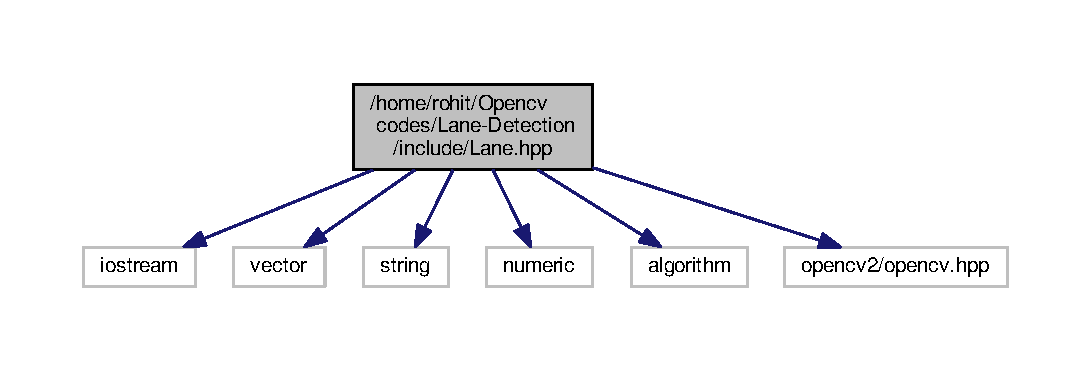
\includegraphics[width=350pt]{Lane_8hpp__incl}
\end{center}
\end{figure}
This graph shows which files directly or indirectly include this file\+:\nopagebreak
\begin{figure}[H]
\begin{center}
\leavevmode
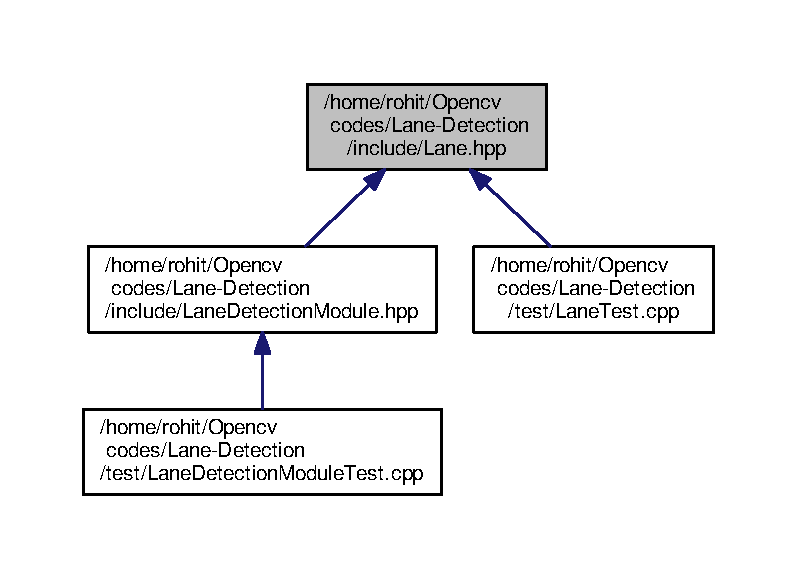
\includegraphics[width=350pt]{Lane_8hpp__dep__incl}
\end{center}
\end{figure}
\subsection*{Classes}
\begin{DoxyCompactItemize}
\item 
class \hyperlink{classLane}{Lane}
\end{DoxyCompactItemize}


\subsection{Detailed Description}
\hyperlink{classLane}{Lane} Detection. 

Copyright 2018 Rohitkrishna Nambiar

\begin{DoxyAuthor}{Author}
rohit517 
\end{DoxyAuthor}
\begin{DoxyDate}{Date}
10/13/2018 
\end{DoxyDate}
\begin{DoxyVersion}{Version}
1.\+0
\end{DoxyVersion}
\hypertarget{LaneTest_8cpp_DESCRIPTION}{}\subsection{D\+E\+S\+C\+R\+I\+P\+T\+I\+ON}\label{LaneTest_8cpp_DESCRIPTION}
Implementation to lane detection system when a video is provided it gives output of Drive heading and lane on video. 
\hypertarget{LaneDetectionModuleTest_8cpp}{}\section{/home/rohit/\+Opencv codes/\+Lane-\/\+Detection/test/\+Lane\+Detection\+Module\+Test.cpp File Reference}
\label{LaneDetectionModuleTest_8cpp}\index{/home/rohit/\+Opencv codes/\+Lane-\/\+Detection/test/\+Lane\+Detection\+Module\+Test.\+cpp@{/home/rohit/\+Opencv codes/\+Lane-\/\+Detection/test/\+Lane\+Detection\+Module\+Test.\+cpp}}


Program to test \hyperlink{classLaneDetectionModule}{Lane\+Detection\+Module} class.  


{\ttfamily \#include $<$gtest/gtest.\+h$>$}\\*
{\ttfamily \#include \char`\"{}Lane\+Detection\+Module.\+hpp\char`\"{}}\\*
{\ttfamily \#include \char`\"{}opencv2/opencv.\+hpp\char`\"{}}\\*
Include dependency graph for Lane\+Detection\+Module\+Test.\+cpp\+:
\nopagebreak
\begin{figure}[H]
\begin{center}
\leavevmode
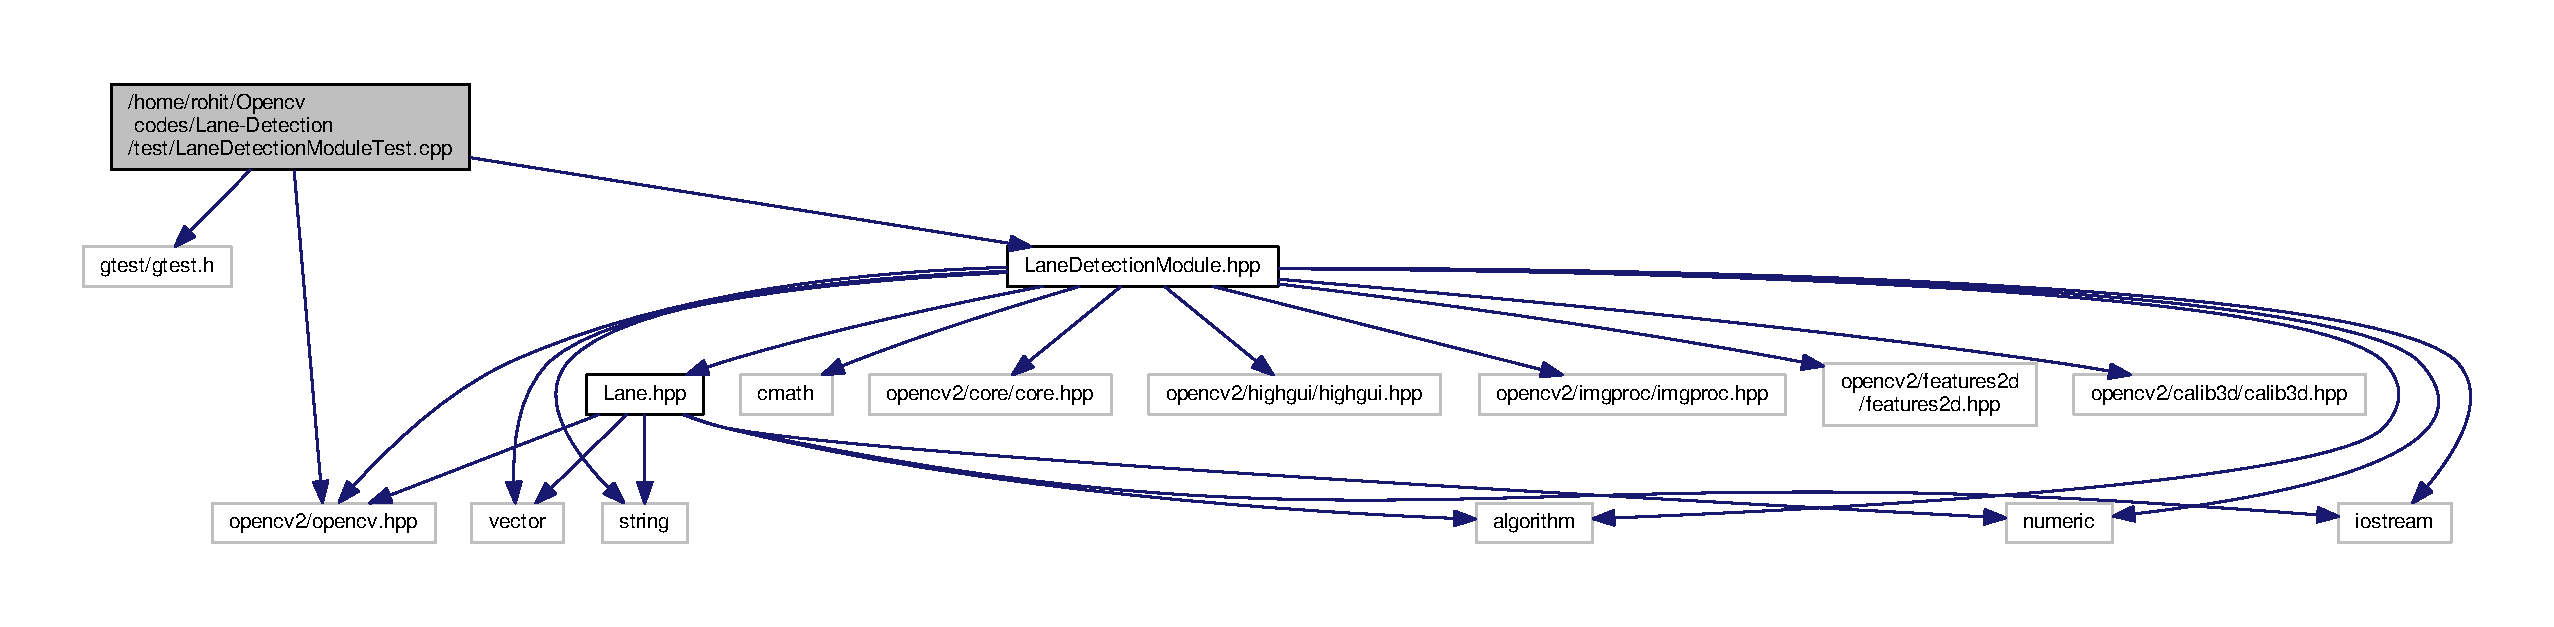
\includegraphics[width=350pt]{LaneDetectionModuleTest_8cpp__incl}
\end{center}
\end{figure}
\subsection*{Functions}
\begin{DoxyCompactItemize}
\item 
\hyperlink{LaneDetectionModuleTest_8cpp_a4c43ba7e450b9290b8e7939a3375279a}{T\+E\+ST} (Get\+Set\+Test, Get\+Gray\+Scale\+Min)
\begin{DoxyCompactList}\small\item\em Test get grey scale min threshold function. \end{DoxyCompactList}\item 
\hyperlink{LaneDetectionModuleTest_8cpp_af149143b44c4f786dccd553f1bfcbe56}{T\+E\+ST} (Get\+Set\+Test, Get\+Gray\+Scale\+Max)
\begin{DoxyCompactList}\small\item\em Test get grey scale max threshold function. \end{DoxyCompactList}\item 
\hyperlink{LaneDetectionModuleTest_8cpp_a42262b2b26165062e43ad46c3547aa30}{T\+E\+ST} (Get\+Set\+Test, Get\+Yellow\+Min)
\begin{DoxyCompactList}\small\item\em Test get yellow min threshold function. \end{DoxyCompactList}\item 
\hyperlink{LaneDetectionModuleTest_8cpp_aaf25ee8b783fdf9722d653ddf05c96d8}{T\+E\+ST} (Get\+Set\+Test, Get\+Yellow\+Max)
\begin{DoxyCompactList}\small\item\em Test get yellow max threshold function. \end{DoxyCompactList}\item 
\hyperlink{LaneDetectionModuleTest_8cpp_ae5c74594ed6121cfe2e1be1f7e2e0348}{T\+E\+ST} (Get\+Set\+Test, Set\+Gray\+Scale\+Min)
\begin{DoxyCompactList}\small\item\em Test set grey min threshold function. \end{DoxyCompactList}\item 
\hyperlink{LaneDetectionModuleTest_8cpp_ae98fab02c4542cec282900fada64c262}{T\+E\+ST} (Get\+Set\+Test, Set\+Gray\+Scale\+Max)
\begin{DoxyCompactList}\small\item\em Test set grey max threshold function. \end{DoxyCompactList}\item 
\hyperlink{LaneDetectionModuleTest_8cpp_a58f6e289a39ee16f0d26aa7a08649e01}{T\+E\+ST} (Get\+Set\+Test, Set\+Yellow\+Min)
\begin{DoxyCompactList}\small\item\em Test set yellow min threshold function. \end{DoxyCompactList}\item 
\hyperlink{LaneDetectionModuleTest_8cpp_ae23653d1b0e1196bbe004816acc148a4}{T\+E\+ST} (Get\+Set\+Test, Set\+Yellow\+Max)
\begin{DoxyCompactList}\small\item\em Test set yellow max threshold function. \end{DoxyCompactList}\item 
\hyperlink{LaneDetectionModuleTest_8cpp_a750e99065b3da187f45a4fb86addb663}{T\+E\+ST} (Functional\+Test, Test\+Image)
\begin{DoxyCompactList}\small\item\em Test for single image execution.. \end{DoxyCompactList}\item 
\hyperlink{LaneDetectionModuleTest_8cpp_a800a31be2c54ea06dd052b71dccebc8f}{T\+E\+ST} (Functional\+Test, Test\+False\+Image\+Path)
\begin{DoxyCompactList}\small\item\em Test for false image path. \end{DoxyCompactList}\end{DoxyCompactItemize}
\subsection*{Variables}
\begin{DoxyCompactItemize}
\item 
\hyperlink{classLaneDetectionModule}{Lane\+Detection\+Module} {\bfseries lane\+Module}\hypertarget{LaneDetectionModuleTest_8cpp_aae7d8ded5d7e5c80095c7654b8ce6bce}{}\label{LaneDetectionModuleTest_8cpp_aae7d8ded5d7e5c80095c7654b8ce6bce}

\end{DoxyCompactItemize}


\subsection{Detailed Description}
Program to test \hyperlink{classLaneDetectionModule}{Lane\+Detection\+Module} class. 

\begin{DoxyAuthor}{Author}
Rohitkrishna Nambiar (rohit517) 
\end{DoxyAuthor}
\begin{DoxyDate}{Date}
10/10/2018 
\end{DoxyDate}
\begin{DoxyVersion}{Version}
1.\+0
\end{DoxyVersion}
\hypertarget{LaneTest_8cpp_DESCRIPTION}{}\subsection{D\+E\+S\+C\+R\+I\+P\+T\+I\+ON}\label{LaneTest_8cpp_DESCRIPTION}
This is a program that tests \hyperlink{classLaneDetectionModule}{Lane\+Detection\+Module} class. 

\subsection{Function Documentation}
\index{Lane\+Detection\+Module\+Test.\+cpp@{Lane\+Detection\+Module\+Test.\+cpp}!T\+E\+ST@{T\+E\+ST}}
\index{T\+E\+ST@{T\+E\+ST}!Lane\+Detection\+Module\+Test.\+cpp@{Lane\+Detection\+Module\+Test.\+cpp}}
\subsubsection[{\texorpdfstring{T\+E\+S\+T(\+Get\+Set\+Test, Get\+Gray\+Scale\+Min)}{TEST(GetSetTest, GetGrayScaleMin)}}]{\setlength{\rightskip}{0pt plus 5cm}T\+E\+ST (
\begin{DoxyParamCaption}
\item[{Get\+Set\+Test}]{, }
\item[{Get\+Gray\+Scale\+Min}]{}
\end{DoxyParamCaption}
)}\hypertarget{LaneDetectionModuleTest_8cpp_a4c43ba7e450b9290b8e7939a3375279a}{}\label{LaneDetectionModuleTest_8cpp_a4c43ba7e450b9290b8e7939a3375279a}


Test get grey scale min threshold function. 


\begin{DoxyParams}{Parameters}
{\em Get\+Set\+Test} & Get set function test \\
\hline
{\em get\+Gray\+Scale\+Min} & Name of the unit test \\
\hline
\end{DoxyParams}
\index{Lane\+Detection\+Module\+Test.\+cpp@{Lane\+Detection\+Module\+Test.\+cpp}!T\+E\+ST@{T\+E\+ST}}
\index{T\+E\+ST@{T\+E\+ST}!Lane\+Detection\+Module\+Test.\+cpp@{Lane\+Detection\+Module\+Test.\+cpp}}
\subsubsection[{\texorpdfstring{T\+E\+S\+T(\+Get\+Set\+Test, Get\+Gray\+Scale\+Max)}{TEST(GetSetTest, GetGrayScaleMax)}}]{\setlength{\rightskip}{0pt plus 5cm}T\+E\+ST (
\begin{DoxyParamCaption}
\item[{Get\+Set\+Test}]{, }
\item[{Get\+Gray\+Scale\+Max}]{}
\end{DoxyParamCaption}
)}\hypertarget{LaneDetectionModuleTest_8cpp_af149143b44c4f786dccd553f1bfcbe56}{}\label{LaneDetectionModuleTest_8cpp_af149143b44c4f786dccd553f1bfcbe56}


Test get grey scale max threshold function. 


\begin{DoxyParams}{Parameters}
{\em Get\+Set\+Test} & Get set function test \\
\hline
{\em get\+Gray\+Scale\+Max} & Name of the unit test \\
\hline
\end{DoxyParams}
\index{Lane\+Detection\+Module\+Test.\+cpp@{Lane\+Detection\+Module\+Test.\+cpp}!T\+E\+ST@{T\+E\+ST}}
\index{T\+E\+ST@{T\+E\+ST}!Lane\+Detection\+Module\+Test.\+cpp@{Lane\+Detection\+Module\+Test.\+cpp}}
\subsubsection[{\texorpdfstring{T\+E\+S\+T(\+Get\+Set\+Test, Get\+Yellow\+Min)}{TEST(GetSetTest, GetYellowMin)}}]{\setlength{\rightskip}{0pt plus 5cm}T\+E\+ST (
\begin{DoxyParamCaption}
\item[{Get\+Set\+Test}]{, }
\item[{Get\+Yellow\+Min}]{}
\end{DoxyParamCaption}
)}\hypertarget{LaneDetectionModuleTest_8cpp_a42262b2b26165062e43ad46c3547aa30}{}\label{LaneDetectionModuleTest_8cpp_a42262b2b26165062e43ad46c3547aa30}


Test get yellow min threshold function. 


\begin{DoxyParams}{Parameters}
{\em Get\+Set\+Test} & Get set function test \\
\hline
{\em get\+Yellow\+Min} & Name of the unit test \\
\hline
\end{DoxyParams}
\index{Lane\+Detection\+Module\+Test.\+cpp@{Lane\+Detection\+Module\+Test.\+cpp}!T\+E\+ST@{T\+E\+ST}}
\index{T\+E\+ST@{T\+E\+ST}!Lane\+Detection\+Module\+Test.\+cpp@{Lane\+Detection\+Module\+Test.\+cpp}}
\subsubsection[{\texorpdfstring{T\+E\+S\+T(\+Get\+Set\+Test, Get\+Yellow\+Max)}{TEST(GetSetTest, GetYellowMax)}}]{\setlength{\rightskip}{0pt plus 5cm}T\+E\+ST (
\begin{DoxyParamCaption}
\item[{Get\+Set\+Test}]{, }
\item[{Get\+Yellow\+Max}]{}
\end{DoxyParamCaption}
)}\hypertarget{LaneDetectionModuleTest_8cpp_aaf25ee8b783fdf9722d653ddf05c96d8}{}\label{LaneDetectionModuleTest_8cpp_aaf25ee8b783fdf9722d653ddf05c96d8}


Test get yellow max threshold function. 


\begin{DoxyParams}{Parameters}
{\em Get\+Set\+Test} & Get set function test \\
\hline
{\em get\+Yellow\+Max} & Name of the unit test \\
\hline
\end{DoxyParams}
\index{Lane\+Detection\+Module\+Test.\+cpp@{Lane\+Detection\+Module\+Test.\+cpp}!T\+E\+ST@{T\+E\+ST}}
\index{T\+E\+ST@{T\+E\+ST}!Lane\+Detection\+Module\+Test.\+cpp@{Lane\+Detection\+Module\+Test.\+cpp}}
\subsubsection[{\texorpdfstring{T\+E\+S\+T(\+Get\+Set\+Test, Set\+Gray\+Scale\+Min)}{TEST(GetSetTest, SetGrayScaleMin)}}]{\setlength{\rightskip}{0pt plus 5cm}T\+E\+ST (
\begin{DoxyParamCaption}
\item[{Get\+Set\+Test}]{, }
\item[{Set\+Gray\+Scale\+Min}]{}
\end{DoxyParamCaption}
)}\hypertarget{LaneDetectionModuleTest_8cpp_ae5c74594ed6121cfe2e1be1f7e2e0348}{}\label{LaneDetectionModuleTest_8cpp_ae5c74594ed6121cfe2e1be1f7e2e0348}


Test set grey min threshold function. 


\begin{DoxyParams}{Parameters}
{\em Get\+Set\+Test} & Get set function test \\
\hline
{\em set\+Gray\+Scale\+Min} & Name of the unit test \\
\hline
\end{DoxyParams}
\index{Lane\+Detection\+Module\+Test.\+cpp@{Lane\+Detection\+Module\+Test.\+cpp}!T\+E\+ST@{T\+E\+ST}}
\index{T\+E\+ST@{T\+E\+ST}!Lane\+Detection\+Module\+Test.\+cpp@{Lane\+Detection\+Module\+Test.\+cpp}}
\subsubsection[{\texorpdfstring{T\+E\+S\+T(\+Get\+Set\+Test, Set\+Gray\+Scale\+Max)}{TEST(GetSetTest, SetGrayScaleMax)}}]{\setlength{\rightskip}{0pt plus 5cm}T\+E\+ST (
\begin{DoxyParamCaption}
\item[{Get\+Set\+Test}]{, }
\item[{Set\+Gray\+Scale\+Max}]{}
\end{DoxyParamCaption}
)}\hypertarget{LaneDetectionModuleTest_8cpp_ae98fab02c4542cec282900fada64c262}{}\label{LaneDetectionModuleTest_8cpp_ae98fab02c4542cec282900fada64c262}


Test set grey max threshold function. 


\begin{DoxyParams}{Parameters}
{\em Get\+Set\+Test} & Get set function test \\
\hline
{\em Set\+Gray\+Scale\+Max} & Name of the unit test \\
\hline
\end{DoxyParams}
\index{Lane\+Detection\+Module\+Test.\+cpp@{Lane\+Detection\+Module\+Test.\+cpp}!T\+E\+ST@{T\+E\+ST}}
\index{T\+E\+ST@{T\+E\+ST}!Lane\+Detection\+Module\+Test.\+cpp@{Lane\+Detection\+Module\+Test.\+cpp}}
\subsubsection[{\texorpdfstring{T\+E\+S\+T(\+Get\+Set\+Test, Set\+Yellow\+Min)}{TEST(GetSetTest, SetYellowMin)}}]{\setlength{\rightskip}{0pt plus 5cm}T\+E\+ST (
\begin{DoxyParamCaption}
\item[{Get\+Set\+Test}]{, }
\item[{Set\+Yellow\+Min}]{}
\end{DoxyParamCaption}
)}\hypertarget{LaneDetectionModuleTest_8cpp_a58f6e289a39ee16f0d26aa7a08649e01}{}\label{LaneDetectionModuleTest_8cpp_a58f6e289a39ee16f0d26aa7a08649e01}


Test set yellow min threshold function. 


\begin{DoxyParams}{Parameters}
{\em Get\+Set\+Test} & Get set function test \\
\hline
{\em set\+Yellow\+Min} & Name of the unit test \\
\hline
\end{DoxyParams}
\index{Lane\+Detection\+Module\+Test.\+cpp@{Lane\+Detection\+Module\+Test.\+cpp}!T\+E\+ST@{T\+E\+ST}}
\index{T\+E\+ST@{T\+E\+ST}!Lane\+Detection\+Module\+Test.\+cpp@{Lane\+Detection\+Module\+Test.\+cpp}}
\subsubsection[{\texorpdfstring{T\+E\+S\+T(\+Get\+Set\+Test, Set\+Yellow\+Max)}{TEST(GetSetTest, SetYellowMax)}}]{\setlength{\rightskip}{0pt plus 5cm}T\+E\+ST (
\begin{DoxyParamCaption}
\item[{Get\+Set\+Test}]{, }
\item[{Set\+Yellow\+Max}]{}
\end{DoxyParamCaption}
)}\hypertarget{LaneDetectionModuleTest_8cpp_ae23653d1b0e1196bbe004816acc148a4}{}\label{LaneDetectionModuleTest_8cpp_ae23653d1b0e1196bbe004816acc148a4}


Test set yellow max threshold function. 


\begin{DoxyParams}{Parameters}
{\em Get\+Set\+Test} & Get set function test \\
\hline
{\em Set\+Yellow\+Max} & Name of the unit test \\
\hline
\end{DoxyParams}
\index{Lane\+Detection\+Module\+Test.\+cpp@{Lane\+Detection\+Module\+Test.\+cpp}!T\+E\+ST@{T\+E\+ST}}
\index{T\+E\+ST@{T\+E\+ST}!Lane\+Detection\+Module\+Test.\+cpp@{Lane\+Detection\+Module\+Test.\+cpp}}
\subsubsection[{\texorpdfstring{T\+E\+S\+T(\+Functional\+Test, Test\+Image)}{TEST(FunctionalTest, TestImage)}}]{\setlength{\rightskip}{0pt plus 5cm}T\+E\+ST (
\begin{DoxyParamCaption}
\item[{Functional\+Test}]{, }
\item[{Test\+Image}]{}
\end{DoxyParamCaption}
)}\hypertarget{LaneDetectionModuleTest_8cpp_a750e99065b3da187f45a4fb86addb663}{}\label{LaneDetectionModuleTest_8cpp_a750e99065b3da187f45a4fb86addb663}


Test for single image execution.. 


\begin{DoxyParams}{Parameters}
{\em Functional\+Test} & Get set function test \\
\hline
{\em Test\+Image} & Name of the unit test \\
\hline
\end{DoxyParams}
\index{Lane\+Detection\+Module\+Test.\+cpp@{Lane\+Detection\+Module\+Test.\+cpp}!T\+E\+ST@{T\+E\+ST}}
\index{T\+E\+ST@{T\+E\+ST}!Lane\+Detection\+Module\+Test.\+cpp@{Lane\+Detection\+Module\+Test.\+cpp}}
\subsubsection[{\texorpdfstring{T\+E\+S\+T(\+Functional\+Test, Test\+False\+Image\+Path)}{TEST(FunctionalTest, TestFalseImagePath)}}]{\setlength{\rightskip}{0pt plus 5cm}T\+E\+ST (
\begin{DoxyParamCaption}
\item[{Functional\+Test}]{, }
\item[{Test\+False\+Image\+Path}]{}
\end{DoxyParamCaption}
)}\hypertarget{LaneDetectionModuleTest_8cpp_a800a31be2c54ea06dd052b71dccebc8f}{}\label{LaneDetectionModuleTest_8cpp_a800a31be2c54ea06dd052b71dccebc8f}


Test for false image path. 


\begin{DoxyParams}{Parameters}
{\em Functional\+Test} & Get set function test \\
\hline
{\em Test\+False\+Image\+Path} & Name of the unit test \\
\hline
\end{DoxyParams}

\hypertarget{LaneTest_8cpp}{}\section{/home/rohit/\+Opencv codes/\+Lane-\/\+Detection/test/\+Lane\+Test.cpp File Reference}
\label{LaneTest_8cpp}\index{/home/rohit/\+Opencv codes/\+Lane-\/\+Detection/test/\+Lane\+Test.\+cpp@{/home/rohit/\+Opencv codes/\+Lane-\/\+Detection/test/\+Lane\+Test.\+cpp}}


Program to test \hyperlink{classLaneDetectionModule}{Lane\+Detection\+Module} class.  


{\ttfamily \#include $<$gtest/gtest.\+h$>$}\\*
{\ttfamily \#include \char`\"{}Lane.\+hpp\char`\"{}}\\*
{\ttfamily \#include \char`\"{}opencv2/opencv.\+hpp\char`\"{}}\\*
Include dependency graph for Lane\+Test.\+cpp\+:
\nopagebreak
\begin{figure}[H]
\begin{center}
\leavevmode
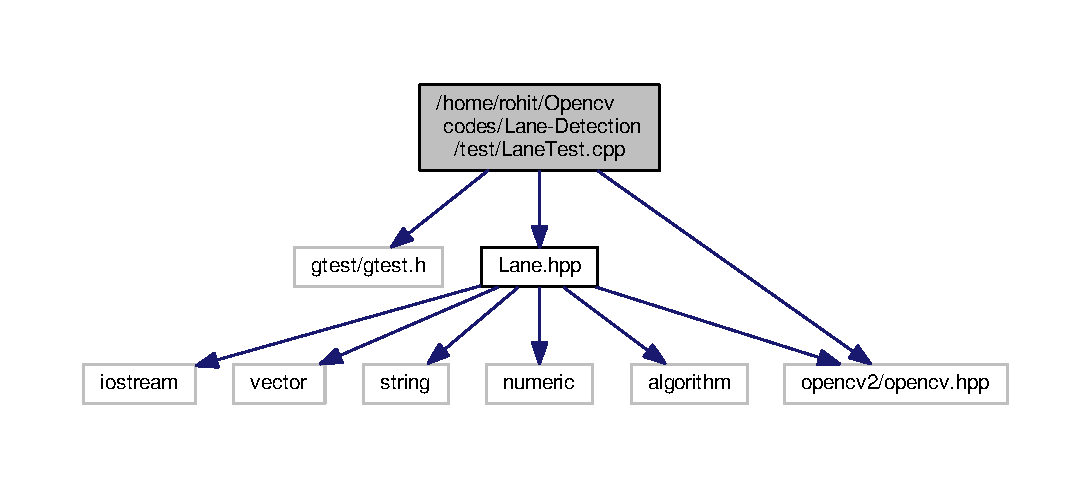
\includegraphics[width=350pt]{LaneTest_8cpp__incl}
\end{center}
\end{figure}
\subsection*{Functions}
\begin{DoxyCompactItemize}
\item 
\hyperlink{LaneTest_8cpp_a33392362c1ed2fdf3fdfd77199b78afd}{T\+E\+ST} (Lane\+Constructor\+Test, Empty\+Constructor)
\begin{DoxyCompactList}\small\item\em \hyperlink{classLane}{Lane} Constructor Test. \end{DoxyCompactList}\item 
\hyperlink{LaneTest_8cpp_a8a08119351ffccd21512701995116e7c}{T\+E\+ST} (Lane\+Constructor\+Test, Custom\+Constructor)
\begin{DoxyCompactList}\small\item\em Custom \hyperlink{classLane}{Lane} Constructor Test. \end{DoxyCompactList}\item 
\hyperlink{LaneTest_8cpp_a25ae68b3530dcae18f78c4280e3e90e2}{T\+E\+ST} (Get\+Set\+Test, poly\+Order\+Get\+Test)
\begin{DoxyCompactList}\small\item\em Poly\+Order getset Test. \end{DoxyCompactList}\item 
\hyperlink{LaneTest_8cpp_a2b5609499a5cf8cf88b1f8b61b91f7b4}{T\+E\+ST} (Get\+Set\+Test, start\+Cood\+Get\+Test)
\begin{DoxyCompactList}\small\item\em Start-\/\+Coordinate getset Test. \end{DoxyCompactList}\item 
\hyperlink{LaneTest_8cpp_a26b3fcfcd4a27d1c6973c68090da76b0}{T\+E\+ST} (Get\+Set\+Test, status\+Get\+Test)
\begin{DoxyCompactList}\small\item\em Status getset Test. \end{DoxyCompactList}\item 
\hyperlink{LaneTest_8cpp_a87e46cbea2841a17100400eeeffd89b7}{T\+E\+ST} (Get\+Set\+Test, poly\+Coeff\+Get\+Test)
\begin{DoxyCompactList}\small\item\em Poly\+Coeff getset Test. \end{DoxyCompactList}\end{DoxyCompactItemize}
\subsection*{Variables}
\begin{DoxyCompactItemize}
\item 
\hyperlink{classLane}{Lane} {\bfseries lane\+Test}\hypertarget{LaneTest_8cpp_aa40b3ce742f2eabea8c54eca79e76576}{}\label{LaneTest_8cpp_aa40b3ce742f2eabea8c54eca79e76576}

\end{DoxyCompactItemize}


\subsection{Detailed Description}
Program to test \hyperlink{classLaneDetectionModule}{Lane\+Detection\+Module} class. 

\begin{DoxyAuthor}{Author}
Rohitkrishna Nambiar (rohit517) 
\end{DoxyAuthor}
\begin{DoxyDate}{Date}
10/10/2018 
\end{DoxyDate}
\begin{DoxyVersion}{Version}
1.\+0
\end{DoxyVersion}
\hypertarget{LaneTest_8cpp_DESCRIPTION}{}\subsection{D\+E\+S\+C\+R\+I\+P\+T\+I\+ON}\label{LaneTest_8cpp_DESCRIPTION}
This is a program that tests \hyperlink{classLaneDetectionModule}{Lane\+Detection\+Module} class. 

\subsection{Function Documentation}
\index{Lane\+Test.\+cpp@{Lane\+Test.\+cpp}!T\+E\+ST@{T\+E\+ST}}
\index{T\+E\+ST@{T\+E\+ST}!Lane\+Test.\+cpp@{Lane\+Test.\+cpp}}
\subsubsection[{\texorpdfstring{T\+E\+S\+T(\+Lane\+Constructor\+Test, Empty\+Constructor)}{TEST(LaneConstructorTest, EmptyConstructor)}}]{\setlength{\rightskip}{0pt plus 5cm}T\+E\+ST (
\begin{DoxyParamCaption}
\item[{Lane\+Constructor\+Test}]{, }
\item[{Empty\+Constructor}]{}
\end{DoxyParamCaption}
)}\hypertarget{LaneTest_8cpp_a33392362c1ed2fdf3fdfd77199b78afd}{}\label{LaneTest_8cpp_a33392362c1ed2fdf3fdfd77199b78afd}


\hyperlink{classLane}{Lane} Constructor Test. 


\begin{DoxyParams}{Parameters}
{\em Constructor\+Test} & Constructor test \\
\hline
{\em Empty\+Constructor} & Name of the unit test \\
\hline
\end{DoxyParams}
\index{Lane\+Test.\+cpp@{Lane\+Test.\+cpp}!T\+E\+ST@{T\+E\+ST}}
\index{T\+E\+ST@{T\+E\+ST}!Lane\+Test.\+cpp@{Lane\+Test.\+cpp}}
\subsubsection[{\texorpdfstring{T\+E\+S\+T(\+Lane\+Constructor\+Test, Custom\+Constructor)}{TEST(LaneConstructorTest, CustomConstructor)}}]{\setlength{\rightskip}{0pt plus 5cm}T\+E\+ST (
\begin{DoxyParamCaption}
\item[{Lane\+Constructor\+Test}]{, }
\item[{Custom\+Constructor}]{}
\end{DoxyParamCaption}
)}\hypertarget{LaneTest_8cpp_a8a08119351ffccd21512701995116e7c}{}\label{LaneTest_8cpp_a8a08119351ffccd21512701995116e7c}


Custom \hyperlink{classLane}{Lane} Constructor Test. 


\begin{DoxyParams}{Parameters}
{\em Constructor\+Test} & Constructor test \\
\hline
{\em Custom\+Constructor} & Name of the unit test \\
\hline
\end{DoxyParams}
\index{Lane\+Test.\+cpp@{Lane\+Test.\+cpp}!T\+E\+ST@{T\+E\+ST}}
\index{T\+E\+ST@{T\+E\+ST}!Lane\+Test.\+cpp@{Lane\+Test.\+cpp}}
\subsubsection[{\texorpdfstring{T\+E\+S\+T(\+Get\+Set\+Test, poly\+Order\+Get\+Test)}{TEST(GetSetTest, polyOrderGetTest)}}]{\setlength{\rightskip}{0pt plus 5cm}T\+E\+ST (
\begin{DoxyParamCaption}
\item[{Get\+Set\+Test}]{, }
\item[{poly\+Order\+Get\+Test}]{}
\end{DoxyParamCaption}
)}\hypertarget{LaneTest_8cpp_a25ae68b3530dcae18f78c4280e3e90e2}{}\label{LaneTest_8cpp_a25ae68b3530dcae18f78c4280e3e90e2}


Poly\+Order getset Test. 


\begin{DoxyParams}{Parameters}
{\em Get\+Set\+Test} & Unit test \\
\hline
{\em poly\+Order\+Get\+Set} & Name of the unit test \\
\hline
\end{DoxyParams}
\index{Lane\+Test.\+cpp@{Lane\+Test.\+cpp}!T\+E\+ST@{T\+E\+ST}}
\index{T\+E\+ST@{T\+E\+ST}!Lane\+Test.\+cpp@{Lane\+Test.\+cpp}}
\subsubsection[{\texorpdfstring{T\+E\+S\+T(\+Get\+Set\+Test, start\+Cood\+Get\+Test)}{TEST(GetSetTest, startCoodGetTest)}}]{\setlength{\rightskip}{0pt plus 5cm}T\+E\+ST (
\begin{DoxyParamCaption}
\item[{Get\+Set\+Test}]{, }
\item[{start\+Cood\+Get\+Test}]{}
\end{DoxyParamCaption}
)}\hypertarget{LaneTest_8cpp_a2b5609499a5cf8cf88b1f8b61b91f7b4}{}\label{LaneTest_8cpp_a2b5609499a5cf8cf88b1f8b61b91f7b4}


Start-\/\+Coordinate getset Test. 


\begin{DoxyParams}{Parameters}
{\em Get\+Set\+Test} & Unit test \\
\hline
{\em start\+Cood\+Get\+Test} & Name of the unit test \\
\hline
\end{DoxyParams}
\index{Lane\+Test.\+cpp@{Lane\+Test.\+cpp}!T\+E\+ST@{T\+E\+ST}}
\index{T\+E\+ST@{T\+E\+ST}!Lane\+Test.\+cpp@{Lane\+Test.\+cpp}}
\subsubsection[{\texorpdfstring{T\+E\+S\+T(\+Get\+Set\+Test, status\+Get\+Test)}{TEST(GetSetTest, statusGetTest)}}]{\setlength{\rightskip}{0pt plus 5cm}T\+E\+ST (
\begin{DoxyParamCaption}
\item[{Get\+Set\+Test}]{, }
\item[{status\+Get\+Test}]{}
\end{DoxyParamCaption}
)}\hypertarget{LaneTest_8cpp_a26b3fcfcd4a27d1c6973c68090da76b0}{}\label{LaneTest_8cpp_a26b3fcfcd4a27d1c6973c68090da76b0}


Status getset Test. 


\begin{DoxyParams}{Parameters}
{\em Get\+Set\+Test} & Unit test \\
\hline
{\em start\+Cood\+Get\+Test} & Name of the unit test \\
\hline
\end{DoxyParams}
\index{Lane\+Test.\+cpp@{Lane\+Test.\+cpp}!T\+E\+ST@{T\+E\+ST}}
\index{T\+E\+ST@{T\+E\+ST}!Lane\+Test.\+cpp@{Lane\+Test.\+cpp}}
\subsubsection[{\texorpdfstring{T\+E\+S\+T(\+Get\+Set\+Test, poly\+Coeff\+Get\+Test)}{TEST(GetSetTest, polyCoeffGetTest)}}]{\setlength{\rightskip}{0pt plus 5cm}T\+E\+ST (
\begin{DoxyParamCaption}
\item[{Get\+Set\+Test}]{, }
\item[{poly\+Coeff\+Get\+Test}]{}
\end{DoxyParamCaption}
)}\hypertarget{LaneTest_8cpp_a87e46cbea2841a17100400eeeffd89b7}{}\label{LaneTest_8cpp_a87e46cbea2841a17100400eeeffd89b7}


Poly\+Coeff getset Test. 


\begin{DoxyParams}{Parameters}
{\em Get\+Set\+Test} & Unit test \\
\hline
{\em start\+Cood\+Get\+Test} & Name of the unit test \\
\hline
\end{DoxyParams}

%--- End generated contents ---

% Index
\backmatter
\newpage
\phantomsection
\clearemptydoublepage
\addcontentsline{toc}{chapter}{Index}
\printindex

\end{document}
